\documentclass[11pt,a4paper]{article}

\usepackage[T1]{fontenc}
\usepackage[utf8]{inputenc}
\usepackage[british]{babel}
\usepackage[left=0mm,right=0mm,top=0mm,bottom=0mm]{geometry}
\usepackage[stretch=25,shrink=25,tracking=true,letterspace=30]{microtype}
\usepackage{graphicx}
\usepackage{xcolor}
\usepackage{marvosym}
\usepackage{enumitem}
\setlist{parsep=0pt,topsep=0pt,partopsep=1pt,itemsep=1pt,leftmargin=6mm}
\usepackage{FiraSans}
\renewcommand{\familydefault}{\sfdefault}
\definecolor{cvblue}{HTML}{304263}

% --- Macros perso ------------------------------------------------------------
\newcommand{\dates}[1]{\hfill\mbox{\textbf{#1}}}
\newcommand{\is}{\par\vskip.5ex plus .4ex}
\newcommand{\smaller}[1]{{\small$\diamond$\ #1}}
\newcommand{\headleft}[1]{\vspace*{3ex}\textsc{\textbf{#1}}\par%
    \vspace*{-1.5ex}\hrulefill\par\vspace*{0.7ex}}
\newcommand{\headright}[1]{\vspace*{2.5ex}\textsc{\Large\color{cvblue}#1}\par%
     \vspace*{-2ex}{\color{cvblue}\hrulefill}\par}

\usepackage[colorlinks=true,urlcolor=white,linkcolor=white]{hyperref}

% -----------------------------------------------------------------------------

\begin{document}
\setlength{\topskip}{0pt}\setlength{\parindent}{0pt}\setlength{\parskip}{0pt}
\setlength{\fboxsep}{0pt}\pagestyle{empty}\raggedbottom

% ============================================================================
%                               COLONNE GAUCHE
% ============================================================================
\begin{minipage}[t]{0.33\textwidth}
\colorbox{cvblue}{\begin{minipage}[t][5mm][t]{\textwidth}\null\hfill\null\end{minipage}}
\vspace{-.2ex}
\colorbox{cvblue!90}{\color{white}
\kern0.09\textwidth
\begin{minipage}[t][293mm][t]{0.82\textwidth}\raggedright
\vspace*{2.5ex}

% ---- Identité ---------------------------------------------------------------
\Large Pape \textbf{\textsc{FALL}} \normalsize

\null\hfill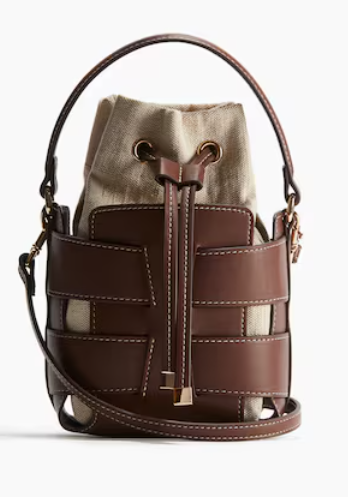
\includegraphics[width=0.65\textwidth]{49a2e5607d8440b7b0c5f743b57afca8.png}\hfill\null

\vspace*{0.5ex}

% ---- Résumé -----------------------------------------------------------------
\headleft{Profile Summary}
Data Scientist avec plus de 2 ans d’expérience dans l’exploitation des données pour créer des produits analytiques à forte valeur ajoutée. Expert en Python, machine learning et visualisation, je conçois des modèles prédictifs robustes, optimise les pipelines de données et communique des insights clairs aux parties prenantes. Passionné par la recherche de solutions innovantes, je combine rigueur scientifique et esprit business pour accélérer la prise de décision.

% ---- Contact ----------------------------------------------------------------
\headleft{Contact details}\small
\MVAt\ {\small pape@gmail.com} \\[0.4ex]
\Mobilefone\ 0753481453 \\[0.5ex]
\Letter\ 12 rue des Data, 75013 Paris, France
\normalsize

% ---- Infos perso ------------------------------------------------------------
\headleft{Personal information}
Citizenship: \textbf{Française} \\[0.5ex]
Family: \textbf{Célibataire} \\[0.5ex]
Languages: \textbf{Français, Anglais}

% ---- Compétences ------------------------------------------------------------
\headleft{Skills}
\begin{itemize}
  \item Python
  \item SQL
  \item Pandas / NumPy
  \item Scikit-learn
  \item TensorFlow / Keras
  \item Machine Learning Supervisé \& Non Supervisé
  \item Deep Learning
  \item Analyse exploratoire de données (EDA)
  \item Visualisation (Matplotlib, Seaborn, Power BI)
  \item Data Engineering (Airflow, Spark)
  \item Docker \& Git
  \item MLOps (MLflow, CI/CD)
\end{itemize}

\end{minipage}\kern 0.09\textwidth
}
\end{minipage}
% ============================================================================
%                               COLONNE DROITE
% ============================================================================
\hskip2.5em
\begin{minipage}[t]{0.56\textwidth}
\setlength{\parskip}{0.8ex}
\vspace{2ex}

% ------------------------ EXPÉRIENCE ----------------------------------------
\headright{Experience}
\textsc{data scientist} at \textit{Prepaya} (Paris, France)  \dates{2022-2023} \\
\smaller{Développé un modèle de scoring client qui a augmenté le taux de conversion de 18 \%}\is
\smaller{Implémenté des pipelines ETL sur Airflow pour automatiser la collecte de données (+4h économisées/jour)}\is
\smaller{Mise en place d’une architecture MLOps (MLflow, Docker, GitHub Actions) réduisant de 30 \% le temps de déploiement}\is
\smaller{Collaboré avec les équipes produit et marketing pour transformer les besoins business en solutions data}\is
\smaller{Présenté les résultats à la direction via des dashboards Power BI interactifs}\is

\textsc{Stagiaire data analyst} at \textit{Edf} (Nanterre, France)  \dates{2023-2024} \\
\smaller{Analyse de séries temporelles de consommation électrique pour prédire les pics de demande (MAPE < 5 \%)}\is
\smaller{Création d’un modèle de classification d’anomalies permettant une détection 40 \% plus rapide des incidents réseau}\is
\smaller{Automatisation de rapports Power BI consultés par 70+ utilisateurs internes}\is
\smaller{Nettoyage et enrichissement de jeux de données brutes (Spark, SQL) de plus de 200 M de lignes}\is
\smaller{Contribution à la stratégie Data \& IA du département R\&D}\is

% ------------------------ ÉDUCATION ----------------------------------------
\headright{Education}
\textsc{Master 2 Data science}. \textit{Sorbonne Université}. \dates{2022-2024} \\

% ------------------------ CERTIFICATIONS ------------------------------------
\headright{Certifications}
\smaller{\textsc{TensorFlow Developer Certificate}}, \textit{Google}. \dates{Mar-2023} \\
\smaller{\textsc{Azure AI Fundamentals}}, \textit{Microsoft}. \dates{Jul-2022} \\

% ------------------------ HOBBIES -------------------------------------------
\headright{Hobbies}
\textit{Musique jazz, Football, Échecs, Photographie urbaine}

\end{minipage}

\end{document}